\documentclass[a4paper]{article}

% Nice way to display code
\usepackage{minted}

% Import images
\usepackage{graphicx}
\usepackage{amsmath}
\usepackage{multicol}

\title{Understanding the connection between
       ranking the internet and eigen vectors}
\author{Vince Knight}
\date{}


\begin{document}
\maketitle

\section{Introduction: The origins of the Page Rank algorithm}

In the early 1990s the internet was becoming popular and there was a need to
find an efficient way of searching \textbf{and finding} web pages for a specific
query. In~\cite{page1999pagerank} Larry Paige, Sergey Brin and Terry Winograd
described an approach they referred to as Page Rank. This became the basis of
the now successful company Google.

In this work, we will describe the problem of ranking web pages with an example,
then go on to describe the basis of the Page Rank algorithm before explaining
how it relates to the eigenvalue of a matrix.

\section{Ranking internet pages}\label{sec:ranking_pages}

The internet can be thought of as a mathematical object called a
graph~\cite{diestel2005graph}.

We can use numpy to generate a random adjacency matrix \(A\) where:

\[
    A_{ij}
    =
    \begin{cases}
        1,&\text{ if }(i,j) \text{ is an edge}\\
        0,&\text{ otherwise}
    \end{cases}
\]

\begin{minted}{python}
>>> size = 10
>>> np.random.seed(0)
>>> A = np.random.choice((0, 1), size=(size, size))
>>> A
array([[0, 1, 1, 0, 1, 1, 1, 1, 1, 1],
       [1, 0, 0, 1, 0, 0, 0, 0, 0, 1],
       [0, 1, 1, 0, 0, 1, 1, 1, 1, 0],
       [1, 0, 1, 0, 1, 1, 0, 1, 1, 0],
       [0, 1, 0, 1, 1, 1, 1, 1, 0, 1],
       [0, 1, 1, 1, 1, 0, 1, 0, 0, 1],
       [1, 0, 1, 0, 1, 0, 0, 0, 0, 0],
       [1, 1, 0, 0, 0, 1, 1, 0, 1, 0],
       [0, 1, 0, 1, 1, 1, 1, 1, 1, 0],
       [1, 1, 0, 0, 1, 0, 0, 1, 1, 0]])
\end{minted}

Each row and column of \(A\) corresponds to a web page (so in our example here
the internet only has 10 web pages). We see that the first web page (the first
row of \(A\) links to all the other webpages except the fourth.

Python has a library for studying networks called networkx. It can be used to
create visualisations:

\begin{minted}{python}
>>> G = nx.from_numpy_array(A, create_using=nx.DiGraph())
>>> plt.figure()
>>> nx.draw(G)
\end{minted}

Figure~\ref{fig:image_of_graph} shows the corresponding network.

\begin{figure}[!hbtp]
    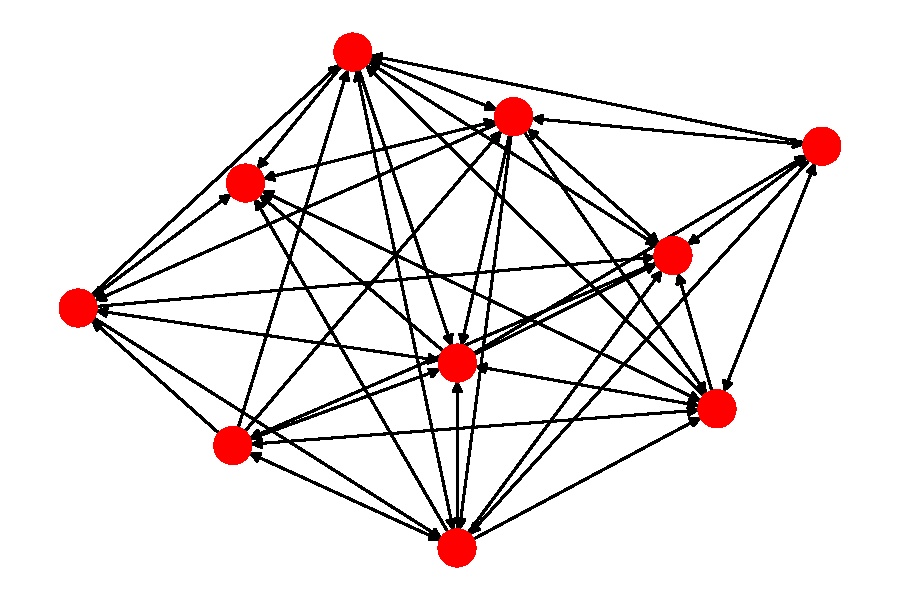
\includegraphics[width=.8\textwidth]{graph.pdf}
    \label{fig:image_of_graph}
\end{figure}

The Page Rank algorithm assumes that users are going to browse the internet in a
random fashion where they are equally likely to go from a page to any of the
other pages that it links to. The score against which it is ranked correspond to
the likelihood of being on a given page:

\begin{minted}{python}
>>> nx.pagerank(G, alpha=1)
{0: 0.11988980099060496,
 1: 0.11337734639341283,
 2: 0.09229073511280955,
 3: 0.08488079369061019,
 4: 0.12554165518523688,
 5: 0.09448445809607922,
 6: 0.09608526108105925,
 7: 0.09314704994034195,
 8: 0.09384213164925923,
 9: 0.08646076786058658}
\end{minted}

\section{Using linear algebra}

We will normalise \(A\) to create a new matrix \(M\) such that the rows all add
to one (so each row give a probability of going to the next page):

\begin{minted}{python}
>>> row_sums = A.sum(axis=1)
>>> M = A / row_sums[:, np.newaxis]
>>> np.round(M, 2)
array([[0.  , 0.12, 0.12, 0.  , 0.12, 0.12, 0.12, 0.12, 0.12, 0.12],
       [0.33, 0.  , 0.  , 0.33, 0.  , 0.  , 0.  , 0.  , 0.  , 0.33],
       [0.  , 0.17, 0.17, 0.  , 0.  , 0.17, 0.17, 0.17, 0.17, 0.  ],
       [0.17, 0.  , 0.17, 0.  , 0.17, 0.17, 0.  , 0.17, 0.17, 0.  ],
       [0.  , 0.14, 0.  , 0.14, 0.14, 0.14, 0.14, 0.14, 0.  , 0.14],
       [0.  , 0.17, 0.17, 0.17, 0.17, 0.  , 0.17, 0.  , 0.  , 0.17],
       [0.33, 0.  , 0.33, 0.  , 0.33, 0.  , 0.  , 0.  , 0.  , 0.  ],
       [0.2 , 0.2 , 0.  , 0.  , 0.  , 0.2 , 0.2 , 0.  , 0.2 , 0.  ],
       [0.  , 0.14, 0.  , 0.14, 0.14, 0.14, 0.14, 0.14, 0.14, 0.  ],
       [0.2 , 0.2 , 0.  , 0.  , 0.2 , 0.  , 0.  , 0.2 , 0.2 , 0.  ]])
\end{minted}

Using this, we can raise \(M\) to a large power to see the long run probability
given starting in any given page.

\begin{minted}{python}
>>> np.round(np.linalg.matrix_power(M, 2000000), 2)
array([[0.12, 0.11, 0.09, 0.08, 0.13, 0.09, 0.1 , 0.09, 0.09, 0.09],
       [0.12, 0.11, 0.09, 0.08, 0.13, 0.09, 0.1 , 0.09, 0.09, 0.09],
       [0.12, 0.11, 0.09, 0.08, 0.13, 0.09, 0.1 , 0.09, 0.09, 0.09],
       [0.12, 0.11, 0.09, 0.08, 0.13, 0.09, 0.1 , 0.09, 0.09, 0.09],
       [0.12, 0.11, 0.09, 0.08, 0.13, 0.09, 0.1 , 0.09, 0.09, 0.09],
       [0.12, 0.11, 0.09, 0.08, 0.13, 0.09, 0.1 , 0.09, 0.09, 0.09],
       [0.12, 0.11, 0.09, 0.08, 0.13, 0.09, 0.1 , 0.09, 0.09, 0.09],
       [0.12, 0.11, 0.09, 0.08, 0.13, 0.09, 0.1 , 0.09, 0.09, 0.09],
       [0.12, 0.11, 0.09, 0.08, 0.13, 0.09, 0.1 , 0.09, 0.09, 0.09],
       [0.12, 0.11, 0.09, 0.08, 0.13, 0.09, 0.1 , 0.09, 0.09, 0.09]])
\end{minted}

We see that all the rows of \(M ^ {2000000}\) are equal and actually correspond to
the values computed using networkx's Page rank.

Interestingly, this set of probabilities can actually be obtained by finding the
right eigenvector of \(M^{T}\):

\begin{minted}{python}
>>> e_values, e_vectors = np.linalg.eig(M.T)
>>> np.real(np.round(e_vectors[:,0] / sum(e_vectors[:,0]), 2))
array([0.12, 0.11, 0.09, 0.08, 0.13, 0.09, 0.1 , 0.09, 0.09, 0.09])
\end{minted}

\section{Conclusion}

The first version of Google's search engine was in fact based on a building
block of linear algebra and graph theory. There are some modifications that
needed to be done to deal with the fact that the internet is not always
completely connected, this corresponds to the \texttt{alpha} argument in the
networkx function above.

\bibliographystyle{plain}
\bibliography{bibliography.bib}

\end{document}
